\section{Neighborhood Analytic}
By its self-describing name, neighborhood analytic aims to provide
summaries of each object over its vicinity. In contrast to the global
analytics which aggregates the entire collection of data as a whole, neighborhood
analytic provides a personalized view on each object per se. Neighborhood
data analytics originates from the window function defined in  SQL which is
illustrated in Figure~\ref{fig:window}.

\begin{figure}[h]
\centering
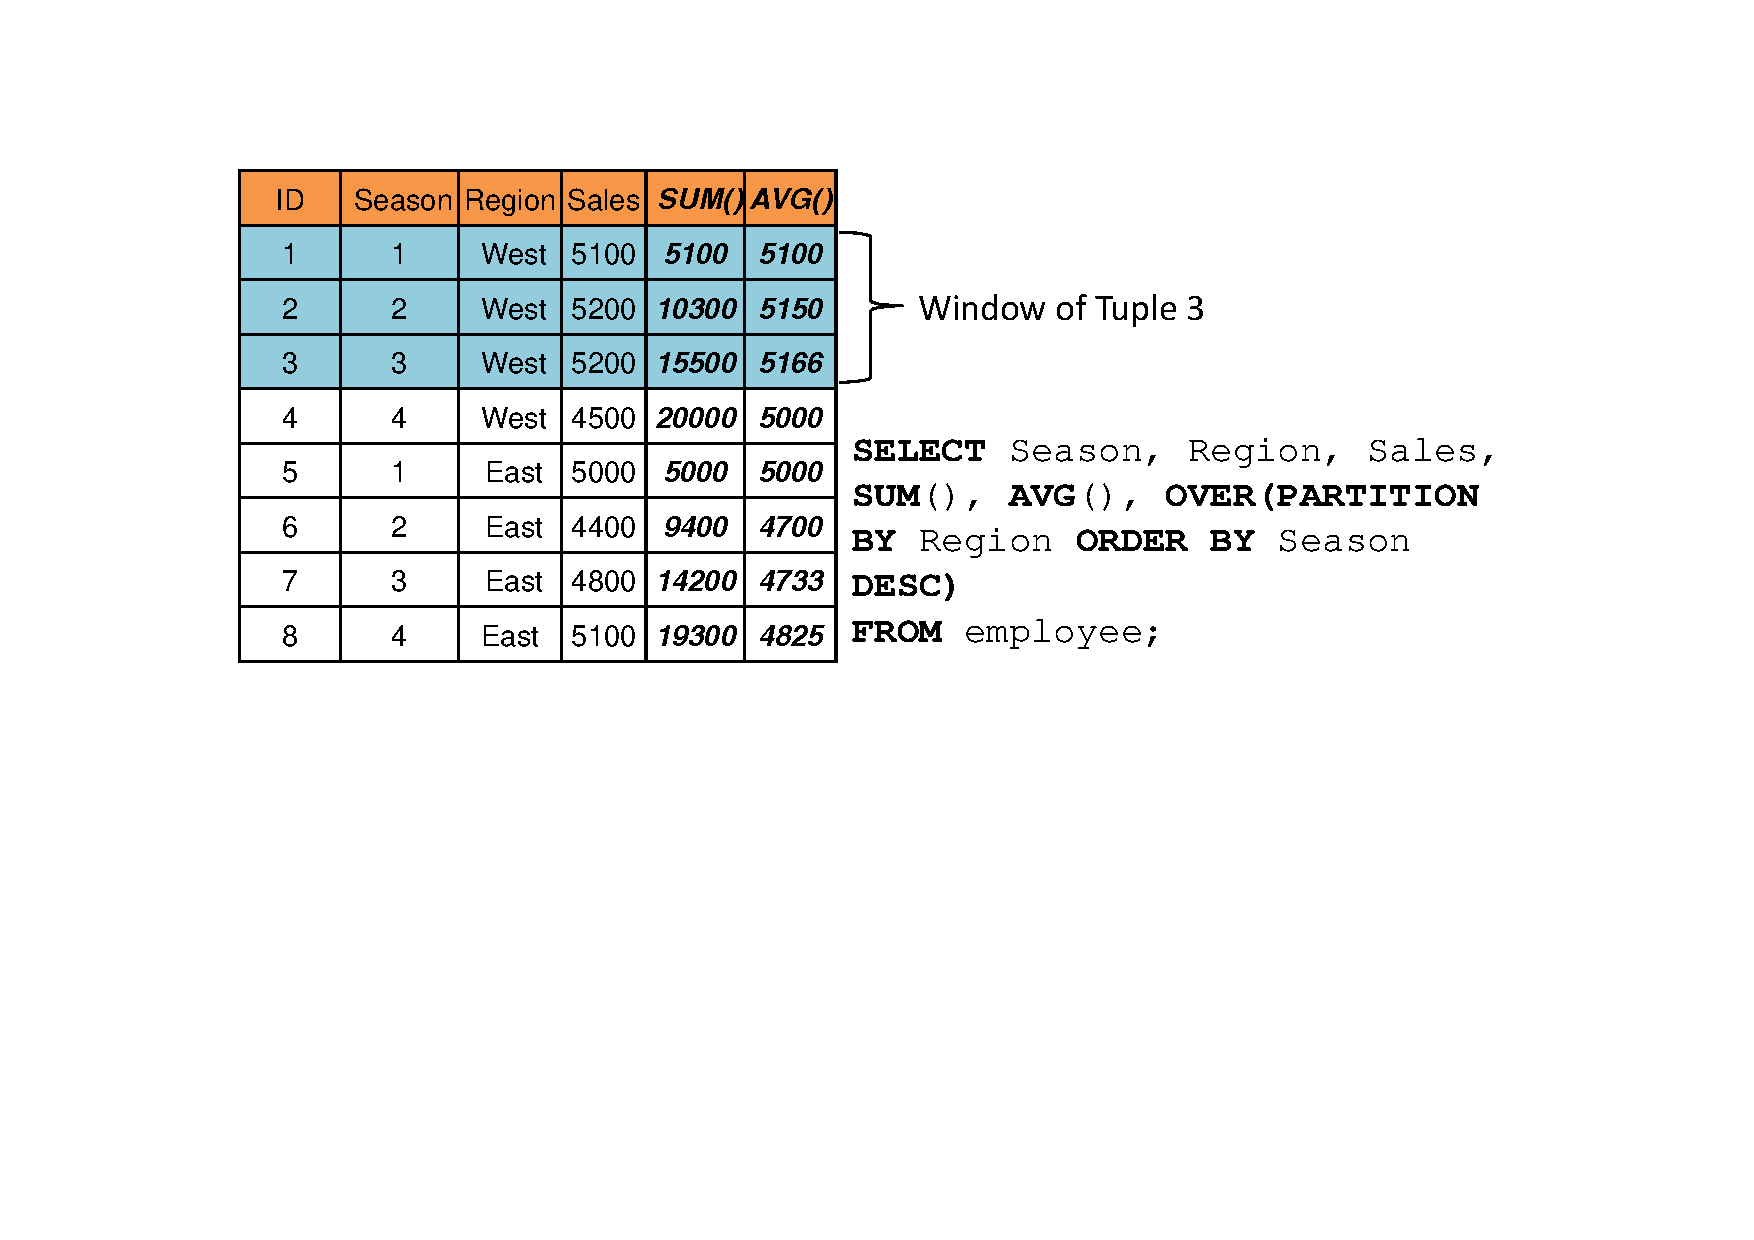
\includegraphics[width=0.8\linewidth]{window_example.pdf}
\caption{A SQL window function computing running sum and average of
sales. The window of season-3 is highlighted.} 
\label{fig:window}
\end{figure}

As shown in the figure, the sales report contains five attributes: 
``Season'', ``Region'' and ``Sales'' are the original fields, ``$\mathtt{sum()}$'' and ``$\mathtt{avg()}$''
are the analytics representing the running sum and average. A window function
is represented by the $\mathtt{over}$ keyword. In this context, the window of a tuple $o_i$
contains other tuples $o_j$ such that $o_i$ and $o_j$ are in the same ``region'' and $o_j$'s ``season'' is
prior to $o_i$'s. The window of season-$3$ for region-``West'' is highlighted.

Apart from this example, there are many other 
usages of the window function in the relational context. 
Being aware of the success of the window function, 
SQL~11 standard incorporates ``$\mathtt{LEAD}$'' and ``$\mathtt{LAG}$'' 
keywords which offer fine-grained specifications on a tuple's window.

Despite the usefulness, there are few works reporting the window
analytics in the non-relational domain. This may dues to the
usage of \emph{sorting} in relational windows. For example,
in Figure~\ref{fig:window},
objects need to be sorted according to ``Season'', and then the window of
each objects is implicitly formed. However, 
in non-relational context, sorting may be ambiguous and even undefined.

To generalize the window function to other domains, we propose the neighborhood
analytics in a broader context. Given a set of objects 
(such as tuples in relational domain or vertexes in graph domain),
the neighborhood analytic is a composite function
$(\mathcal{F} \circ \mathcal{N})$ applied on every object. $\mathcal{N}$
is the \emph{neighborhood function}, which contains the related objects of an object;
$\mathcal{F}$ is an \emph{analytic function}, which could be aggregate, rank,
pattern matching, etc.
Apparently, the relational window function is a special case of the
neighborhood analytics. For example, window function in Figure~\ref{fig:window} 
can be represented as $\mathcal{N}(o_i)=\{o_j | o_i.season > o_j.season \wedge o_i.region = o_j.region\}$
and $\mathcal{F} = \mathtt{avg}$.
Since the \emph{sorting} requirement is relaxed, our neighborhood analytics could
enrich the semantic of relational window notations 
and can be applied on other domains.